\documentclass[a4,12pt]{article}
\usepackage[utf8]{inputenc}
\usepackage[spanish]{babel}
\usepackage[margin=3cm]{geometry}
\usepackage{graphicx}
\usepackage{import}
\usepackage{color}
%\usepackage{times}

\renewcommand{\familydefault}{\sfdefault}


\usepackage{hyperref}

\hypersetup{
    pdfborder = {0 0 0}
}

\title{Trabajo para el departamento de DIS \newline
\LaTeX, GIT y Octave}

\author{Óscar Berrocal Fráhija}



\begin{document}

\maketitle



\begin{abstract}
Este documento tratará de desarrollar un pequeño trabajo en GNU Octave, documentándolo en latex y usando git como repositorio. En paticular, evaluaré el rendimiento de un algoritmo sencillo sobre matrices, que se corresponde a la parte matemática de uno de los efectos cláscios de la demoscene.
\end{abstract}

\tableofcontents

\listoffigures

\newpage

\section{Introducción}
La demoscene es una subcultura del arte por ordenador que se especializa en la producción de demos, que son presentaciones audiovisuales con gráficos y sonido generados en tiempo real por el ordenador.
\newline
\newline
Antes del auge de los IBM PC, los ordenadores personales contaban con un hardware poco variado y configurable, existiendo unas limitaciones y características bien conocidas. Grupos de crackers y artistas gráficos por igual trataban de producir toda clase de efectos gráficos y sonoros llevando al límite las capacidades del hardware existente, superando en sus intros con creces lo que grandes compañías de videojuegos eran capaces de producir.
\newline
\newline
\begin{figure}[h!]
  \centering
    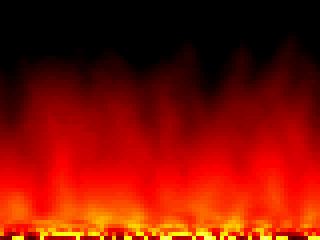
\includegraphics{img/fire}
  \caption{Aspecto del efecto clásico de fuego}
\end{figure}
En la época en que ordenadores tales como el commodore 64, Amiga o Amstrad CPC copaban el mercado, las limitaciones conocidas del hardware permitían implementar de forma precisa este tipo de efectos, creándose un catálogo de conocidos efectos clásicos de la demoscene, como fuego, plasma, túneles, y deformaciones basadas en funciones trigonométricas.
\newline
\newline
\begin{figure}[h!]
  \centering
    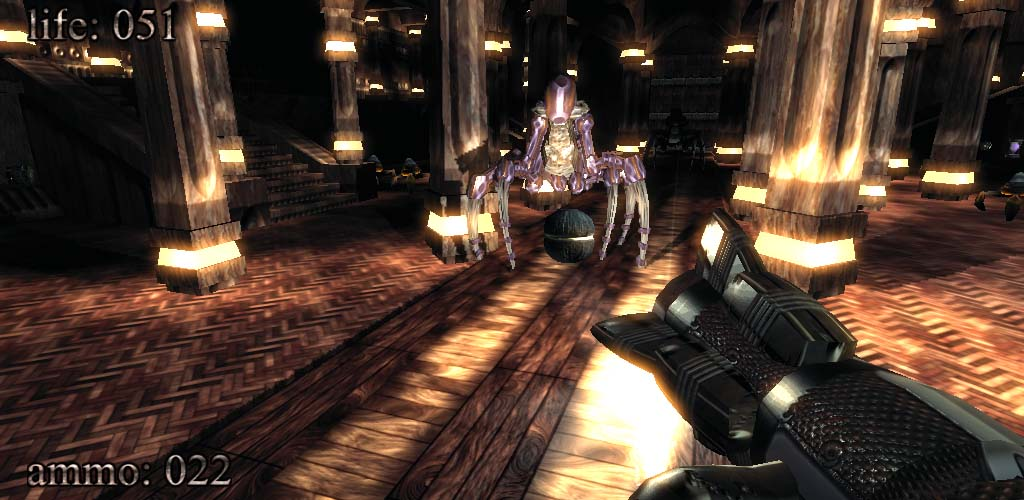
\includegraphics[scale=0.5]{img/kkrieger}
  \caption{.kkrieger, juego completo generado proceduralmente en 96KB}
\end{figure}
Posteriormente, cuando los PC compatibles se asentaron y su hardware fue diversificándose y siendo cada vez más potente, estas restricciones fueron desapareciendo, y en su lugar se trató de generar presentaciones procedurales lo más avanzadas posible tratando de mantener restricciones artificialmente, por ejemplo en el tamaño máximo de los ejecutables.
\newline
\newline
Un ejemplo de ello sería kkrieger, desarrollado por el grupo .theprodukt en 2004, que consigue implementar un juego completo de acción en primera persona en tan sólo 96KB, generando en tiempo real modelos, texturas, niveles y sonido.


\begin{figure}[h!]
  \centering
    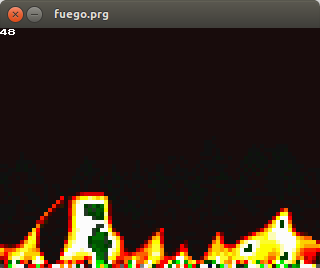
\includegraphics{img/fuego}
  \caption{Otra implementación del mismo efecto, sin buffer}
\end{figure}


\subsection{El efecto de fuego}
De entre los efectos disponibles, he elegido uno relativamente sencillo y fácil de medir. El efecto de fuego que puede verse en la figura 1, trabaja sobre una matiz, haciendo operaciones matemáticas sencillas. En los primeros PCs compatibles, era muy común el modo 13 de vídeo, que ofrecía una resolución de 320x200 pixel y 8 bits de profundidad de color (256 colores). Ajustando dicha paleta de colores a un degradado de tonos de rojos, naranjas y amarillos, de más oscuro a más claro (siendo el cero el negro, y el 255 el color más brillante), podemos definir una matriz de 320x200 bytes, cuyas posiciones se corresponden con píxeles de pantalla en el modo de vídeo, y el valor de cada posición con el color que se muestra en dicha posición.
\newline
\newline
En cada fotograma, la fila inferior de la matriz (o pantalla) se rellena de números aleatorios, y se hace un recorrido al resto de la matriz, calculando su valor como el promedio entre los puntos colindantes:\newline
[tex]punto[x,y] = (punto[x-1,y] + punto[x+1,y] + punto[x,y-1] + punto[x,y+1]) / 4;[/tex] \newline
Se trata realmente de un filtro de suavizado de imagen, tomando como imagen el fotograma anterior y una fila inferior de números aleatorios (que sería la fuente de las llamas).
\newline
\newline
El alcance de este trabajo no es la implementación de una intro funcional, sino de la simulación en octave de los cálculos realizados por el efecto en cuestión para distintos tamaños de problema (cálculo en distintos tamaños de matriz), con el fin de comprobar si es posible obtener una tasa aceptable de fotogramas por segundo.

\section{Desarrollo}

Explicaremos todo aquí.

\subsection{Sub1}

Adios.

\subsection{Sub2}

Hola.


%\bibliographystyle{plain}
%\bibliography{referencias}

\end{document}

